\documentclass[a4paper]{article}
\usepackage[utf8]{inputenc}
\usepackage{kotex}
\usepackage{fancyhdr}
\usepackage{amsmath}
\usepackage{amssymb}
\usepackage{indentfirst}
\usepackage{amsthm}
\usepackage{algpseudocode}
\usepackage{algorithm}
\usepackage{graphicx}
\usepackage{appendix}

\newcommand{\Leg}[3][]{\left(\frac{#2}{#3}\right)_{#1}}
\newtheorem{lemma}{Lemma}
\newtheorem{theorem}{Theorem}
\newtheorem{definition}{Definition}
\pagestyle{fancy}
\fancyhf{}
\lhead{Construction of the perfect-square detection heuristic}
\rhead{R\&E 중간 보고서}
\rfoot{Page \thepage}

\begin{document}
    \begin{titlepage}
        \centering
	    %\includegraphics[width=0.15\textwidth]{example-image-1x1}\par\vspace{1cm}
	    {\scshape\LARGE Kangwon Science Highschool \par}
	    \vspace{1cm}
	    {\scshape\Large A novel $O(|P|k\max_{p_i \in P}{p_i})$-time heuristic\par}
        \vspace{1.5cm}
	    {\huge\bfseries Construction of the perfect-square number detection heuristic\par}
	    \vspace{2cm}
	    {\Large\itshape Kim Jun Hyeok\par}
	    \vfill
	    {\large \today\par}
    \end{titlepage}
    \linespread{1.5}
    \begin{abstract}
        기존에 이분 탐색과 산술(Arithmetic) 연산을 이용하여 제시되었던 $k$-bit 정수에 대하여 $O(k^{3})$혹은 $O(k^{2}\log{k})$시간 결정론적 알고리즘은 매우 큰 수에 대해서는 시간이 오래 걸리는 결점이 있다.
        이 연구에서는, 빅데이터 분석을 통해서 임의의 홀수인 소수에 관한 이차 잉여(Quadratic-residue)에 대하여 Euler’s criterion 을 이용한 완전 제곱수 휴리스틱(Heuristic) 제시와 유의미한 높은 확률로 판정 가능한 소수들의 최소 개수를 제시하는 것을 목표로 한다. 
        또한, 후속 연구 방안으로 임의의 제곱수를 비트로 표현하였을 때 임의의 개수의 제곱수에 관하여 LCS(Longest-common- sequence)를 구하여 여기에서 찾은 LCS 를 통해서 매칭하는 휴리스틱을 제시하고, 위의 방법과 결합하여 더욱 판정률을 높인다.
    \end{abstract}
    \addcontentsline{toc}{section}{참고 문헌}
    \tableofcontents
    \newpage
    \section{서론}
        기존에 제시된 결정론적 다항 시간(Deterministic polynomial time)에 임의의 $k$-bit 정수가 제곱수(Perfect-square number)인지 결정하는 알고리즘은, 이분 탐색(Binary search)와 산술 연산(Arithmetic operation)을 통해서 $O(k^{2})$ Naïve 정수 곱셈을 이용하면, $O(k^{3})$시간에 결정할 수 있다.
        여기에서, Fürer 의 $O(k\log{k})$ 시간 정수 곱셈 알고리즘을 이용하면, $O(k^{2}\log{k})$시간에 문제를 해결할 수 있다. \cite{fürer_2007}
        하지만 $k$의 크기가 매우 커지면 수행이 느려지는 결점이 있다. \\
        이 연구에서는 이를 개선시킬, $k=10^{8}$, $N=10^{10^{8}}$에서도 빠른 수행시간이 보장되는 $k$에 대하여 선형 시간에 가까운 휴리스틱을 제시한다. \\
        또한, 임의의 홀수인 소수 $p$에 대하여 다음과 같은 Euler’s criterion을 통해서 $a \in GF(p)$에 대하여 Legendre’s symbol 을 계산할 수 있다. \cite{hardy_heath-brown_wright_2011}
        \[
            \Leg{a}{p} \equiv a^{\frac{p-1}{2}} \text{ (mod p)}
        \]
        여러 소수에 대하여 반복적으로 시도해봄으로서 높은 확률로 제곱수임을 판정할 수 있다.
        본 연구에서는 임의의 $k$-bit 정수가 제곱수(Perfect-square number)인지 결정하는 $O(k\log{k})$시간 휴리스틱을 제시한다.
    \section{본론}
    \subsection{이론적 배경}
        이차 잉여(Quadratic)를 통한 확률적인 알고리즘을 설계하기 위해서 다음과 같은 정의가 필요하다.
        \begin{definition}
            임의의 홀수인 소수 $p$와 $a \in GF(p)$에 대하여 $a$가 $p$에 대한 이차 잉여(Quadratic residue)라는 것은
            $x^{2} \equiv a \ (mod \ p)$인 $x \in GF(p)$가 존재하는 것이다.
        \end{definition}
        \begin{definition}
            임의의 홀수인 소수 $p$와 $a \in GF(p)$에 대하여 Legendre's symbol은 다음과 같이 정의된다.
            \begin{equation}
                \Leg{a}{p} \equiv 
                \begin{cases}
                    1 & \text{a is a quadratic residue of p}\\
                    -1 & \text{Otherwise}
                \end{cases}
            \end{equation}
        \end{definition}
        \begin{theorem}
            \label{thm1}
            임의의 홀수인 소수 $p$와 $a \in GF(p)$에 대하여 다음과 같은 식이 성립한다.
            \begin{equation}
                \Leg{a}{p} \equiv a^{\frac{p-1}{2}} \text{ (mod p)}
            \end{equation}
        \end{theorem}
        \begin{proof}
            Hardy, G. H., et al., \textit{An introduction to the Theory of numbers (Sixth ed.)} \cite{hardy_heath-brown_wright_2011}를 참고하라.
        \end{proof}
        \begin{theorem}
            $GF(p)$에서 홀수인 소수 $p$에 대한 이차 잉여의 개수는 $\frac{p-1}{2}$이다.
        \end{theorem}
        \begin{proof}
            만일 $n,m \in GF(p)$에 대하여 $n^{2} \equiv m^{2}$을 만족하려면, $n \equiv -m$ 또는 $n \equiv m$을 만족하여야 한다.
            따라서 $n^{2} \text{ mod p}$의 서로 다른 결과는 최대 $\frac{p-1}{2}$개가 될 수 있다. 따라서 성립한다.
        \end{proof}
    \subsection{알고리즘 설계}
        임의의 홀수인 소수 $p$와 $a \in GF(p)$에 대하여, $\Leg{a}{p}$를 계산하는 것은 \ref{thm1}과 분할-정복 기법(Divide-and-conquer method)을 통한 거듭 제곱과 Fürer의 곱셈 알고리즘 등을 이용하여 $O(\log{p}\log{\log{p}})$시간에 계산할 수 있다.
        \begin{algorithm}
            \caption{Legendre's symbol heuristic}\label{algo1}
            \begin{algorithmic}
                \State $p \gets \text{RandomPrime()}$
                \State $m \gets \text{Pow(a,$\frac{p-1}{2}$,p)}$
                \If {$m == 1$}
                    \State \textbf{return} true
                \Else
                    \State \textbf{return} false
                \EndIf
            \end{algorithmic}
        \end{algorithm}
        여기에서, $Pow(a,x,p)$는 $a \text{ mod p}$를 분할-정복 기법을 통해서 충분히 작은 $p$에 대하여 $O(\log{p})$시간에 계산하는 함수이다.
        다음과 같은 정리를 이용하여 통계학적인 분류에 중요한 영향을 끼치게 될 것이다.
        \begin{lemma}
            임의의 제곱수 $n^{2}$과 홀수인 소수 $p$에 대하여 $\Leg{n^{2}}{p} \equiv 1$이다.
        \end{lemma}
        \begin{proof}
            \ref{thm1}과 Fermat's little theorem \cite{hardy_heath-brown_wright_2011}에 의하여 $\Leg{n^{2}}{p}\equiv n^{p-1} \equiv 1 \text{ (mod p)}$가 성립한다.
        \end{proof}
        따라서 우리는 임의의 제곱수가 아닌 수에 대하여 어떤 홀수인 소수 $p$의 이차 잉여가 되는 경우를 확인하면 된다.
        그리고, 이 과정에서 $K$개의 소수를 선택하도록 하자.
        그리고 이 소수들의 집합을 $P$라고 하자.
        여기에서 정상적인 판단이 안되는 두 가지의 경우가 있다.
        \begin{enumerate}
            \item $p_{i} \in P$가 $p_{i} \mid a$인 경우이다. 여기에서 모든 수에 대하여 이러한 상황을 만족할 확률은 약 $\frac{1}{\prod\nolimits_{i} p_{i}}$이다.
            \item $a$가 완전 제곱수가 아니고, $\Leg{a}{p_{i}} \equiv 1$를 만족하는 경우이다.
        \end{enumerate}
        두번째 경우에 대해서 $a = m^{2} \equiv d_{i} \text{ (mod p)}$, $n_{1} = p_{i} + b \rightarrow n_{1}^{2}=p_{i}(p_{i} + 2b) + b^{2}$이고,
        $n_{1}^{2} = p_{i}k + c$, $c < p_{i}$ 꼴로 나타내어지기 원하니 이런 $k$의 기댓값은 $p_{i} > 9$를 가정하여,
        $c$가 $\sqrt{p}$를 넘을 확률은 약 $\frac{p_{i} - \sqrt{p_{i}}}{p_{i}}$이고 이 경우에는 $k=p_{i} + 2b + 1$이니 $k$의 기댓값을 근사하면,
        $k_{expect}=\frac{1}{p_{i}}(p_{i} + 2b_{expect}) + \frac{p_{i} - \sqrt{p_{i}}}{p_{i}}(p_{i} + 2b_{expect} + 1)=p_{i} + 2b_{expect} + 1 - \frac{1}{\sqrt{p_{i}}} \approxeq p_{i} + 2b_{expect} + 1$이다. \\
        또한, $b$의 기댓값을 근사하면, $b_{expect} = \frac{1}{\sqrt{p_{i}}} \sqrt{d_{i}} + \frac{p_{i} - \sqrt{p_{i}}}{p_{i}} (\sqrt{d_{i}} - p_{i}) = \frac{1}{\sqrt{p_{i}}}\sqrt{d_{i}} + \sqrt{d_{i}} - p_{i} - \frac{1}{\sqrt{p_{i}}}(\sqrt{d_{i}} - p_{i}) = \sqrt{d_{i}} - p_{i} + \sqrt{p_{i}}$이다.
        결국 고정된 $a$에 대하여 단위 구간 $[1,n_{1}^{2}]$에서는 약 $p_{i} + 2b_{expect} - 1 = p_{i} + 2\sqrt{d_{i}} - 2p_{i} + 2\sqrt{p_{i}} - 1 = 2(\sqrt{d_{i}} + \sqrt{p_{i}}) - (p_{i} + 1)$개의 위 조건을 만족하지 않고 $d_{i}$와 합동인 수가 존재한다. \\
        따라서 $a \geq p_{i} + d_{i}$이고 $[1,a]$에 대하여 위와 같은 조건을 만족하는 수의 개수는 약 $\frac{a(2(\sqrt{d_{i}} + \sqrt{p_{i}}) - p_{i})}{p_{i}(p_{i}+2\sqrt{d_{i}}-p_{i}+\sqrt{p_{i}})}$개가 존재한다.
        따라서 약 $\frac{2(\sqrt{d_{i}} + \sqrt{p_{i}}) - p_{i}}{p_{i}(2(\sqrt{d_{i}} + \sqrt{p_{i}}) - (p_{i} + 1))}$의 확률로 고정된 $d_{i}$에 대하여 정확히 판정할 수 없게 된다.
        \begin{equation}
            Pr(p_{i}) = \frac{1}{p_{i}}(1 + \sum_{d_{i}=1}^{p_{i}-1} \frac{2(\sqrt{d_{i}} + \sqrt{p_{i}}) - p_{i}}{2(\sqrt{d_{i}} + \sqrt{p_{i}}) - (p_{i} + 1)})
        \end{equation}
        여기에서 $\forall p_{i} \in P$에 대하여 실패할 확률은 $\prod\nolimits_{p_{i} \in P} Pr(p_{i})$이니 $|P|$가 커질 수록 더 줄어든다.
        또한, $p_{i}$가 커질 수록 더 줄어든다.
        이 결과의 가장 큰 의미는 구간에 상관 없이 확률이 균등하다는 것이다.
        따라서 적절하게 각 $p_{i}$와 $|P|$를 선택하면 충분히 낮은 오류로 \ref{algo1}에 따른 제곱수를 판정할 수 있다.
        \begin{figure}[h]
            \centering
            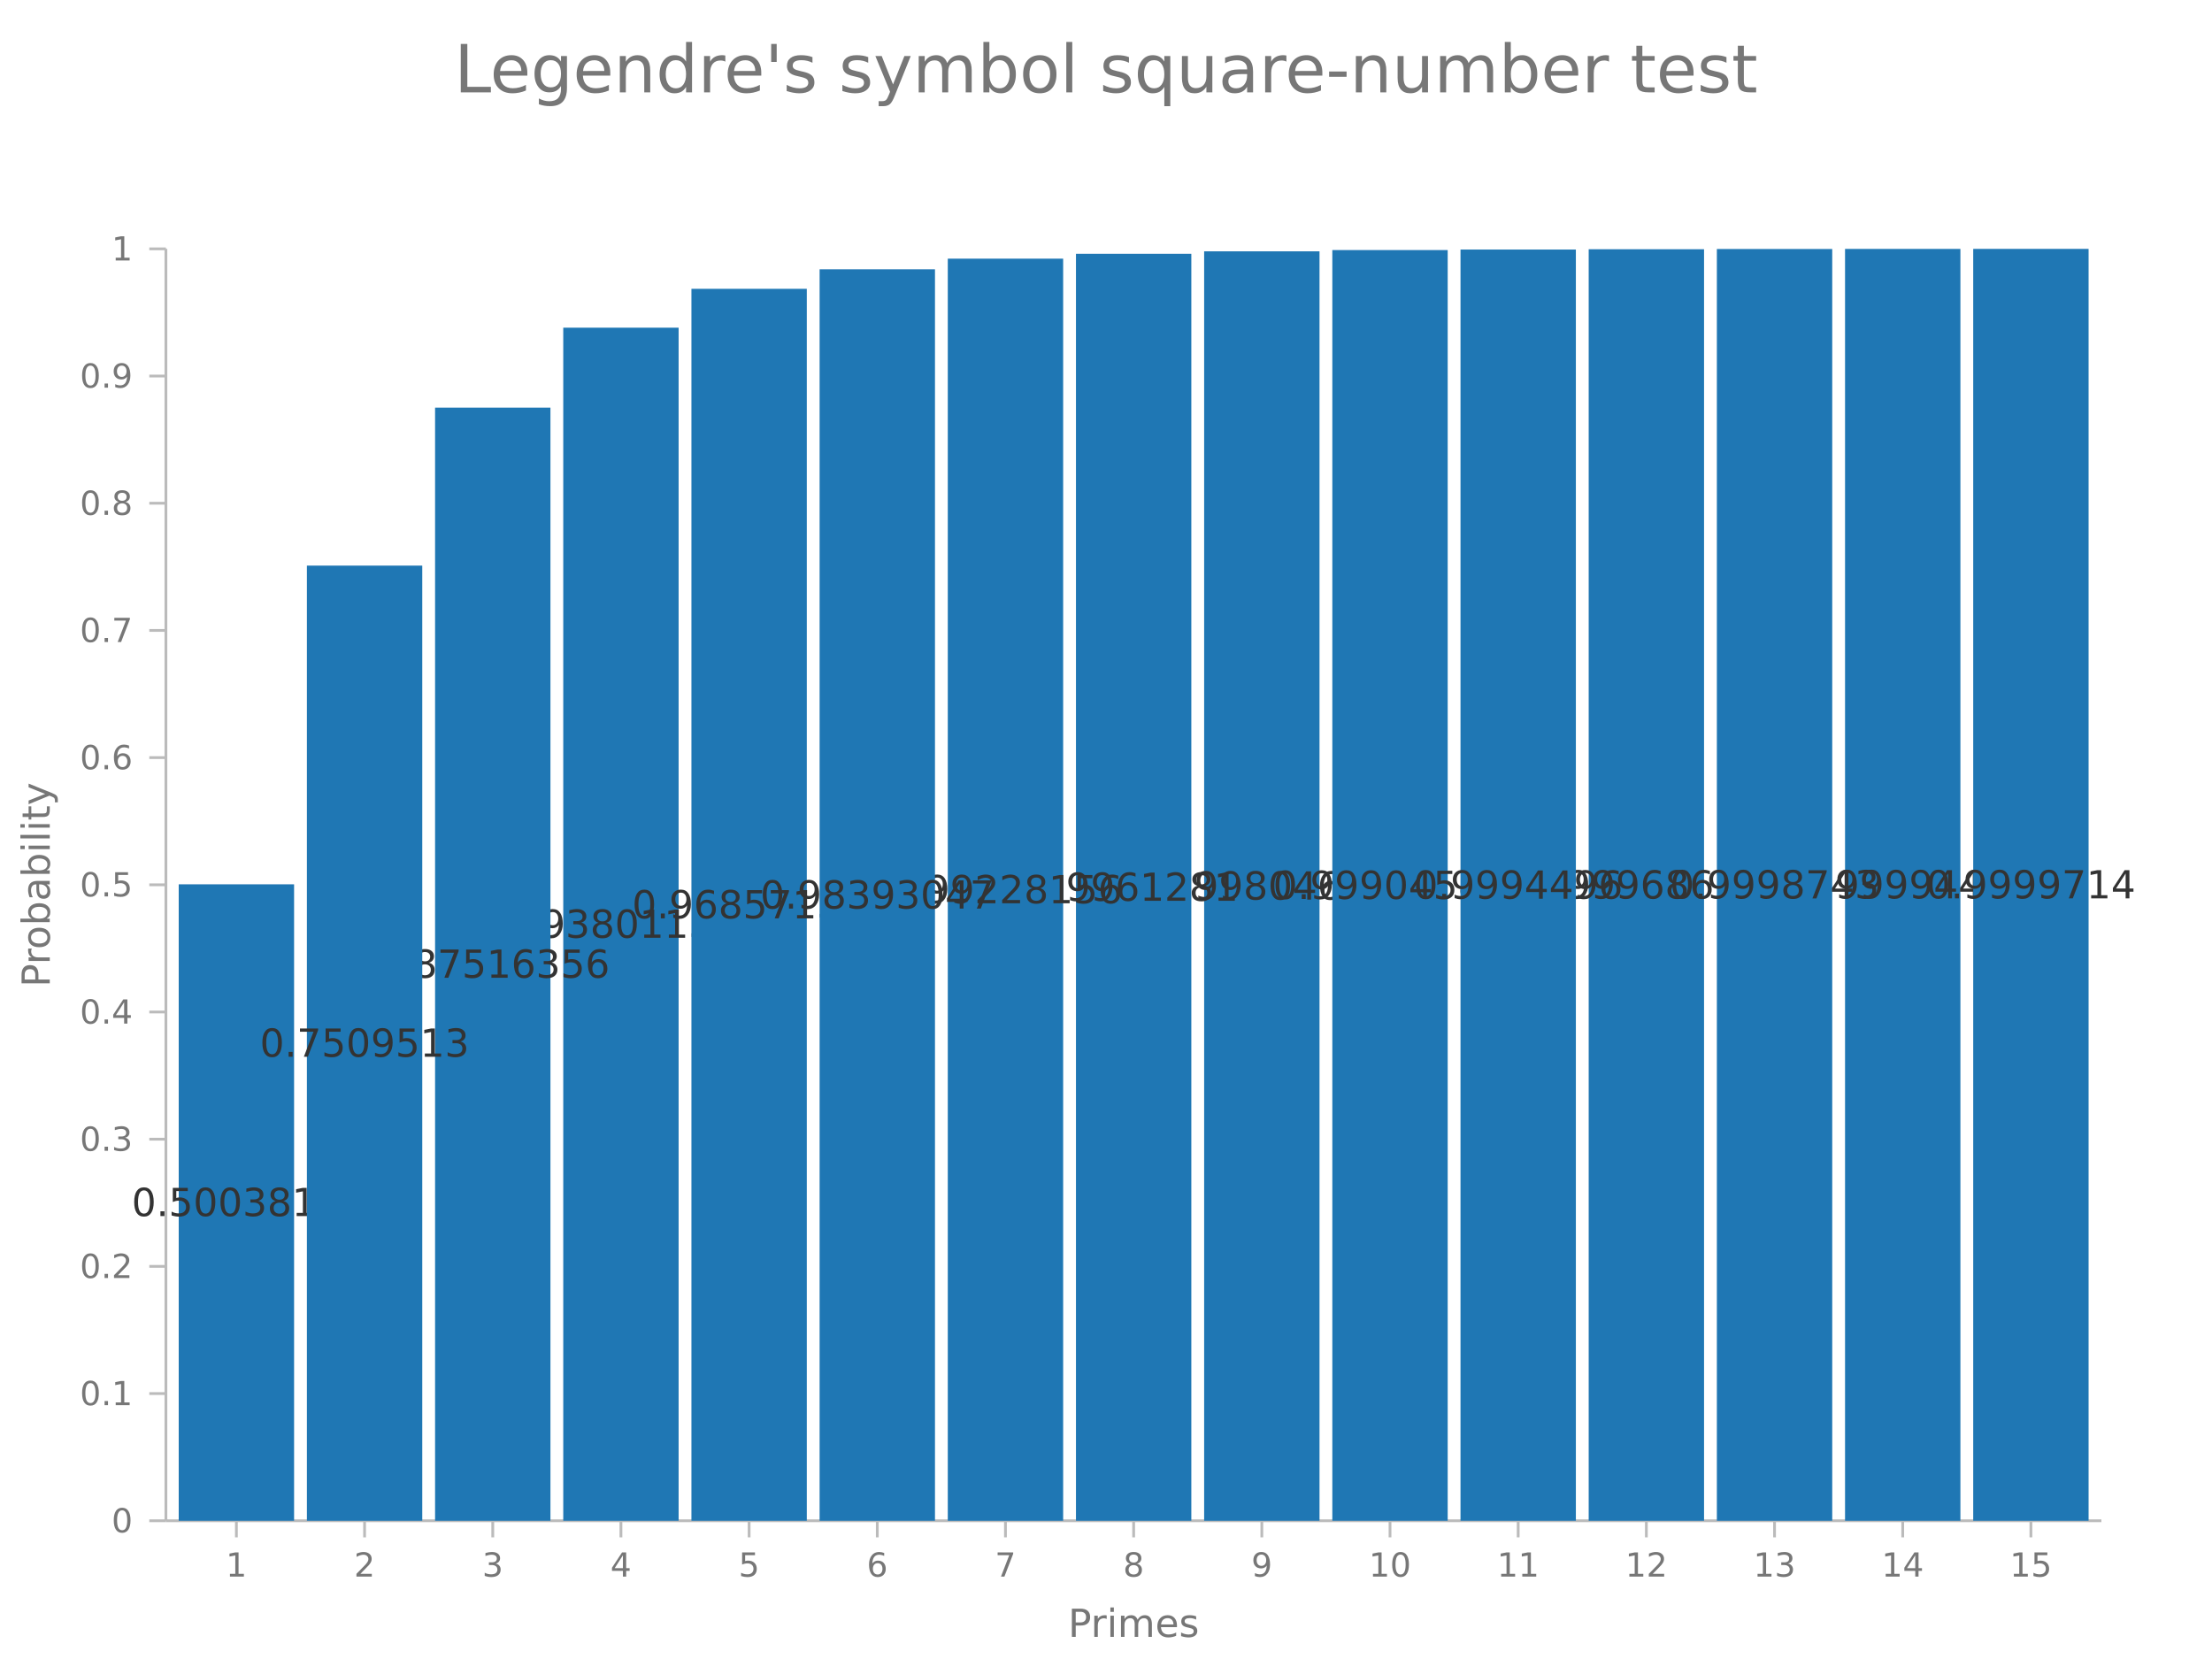
\includegraphics[width=\textwidth]{legendre-test.png}
            \caption{$|P|$의 변화 따른 성공 확률을 나타낸 히스토그램. $[1,10^{6}]$ 구간에서 랜덤한 소수에 대하여 확인하였다.}
            \label{fig1}
        \end{figure}
        \ref{fig1}에 따르면 machine epsilon $\epsilon = 10^{-3}$이라고 가정할때 $|P|=10$정도가 수행 시간등의 측면에서 적절하다고 볼 수 있다.
        또한, 충분히 큰 랜덤한 소수로 잡는 것으로 충분하다.
        여기에서 사용된 코드는 부록에 있는 링크에 존재한다.
        또한, 데이터 분석을 통해서 $|P|$가 일정할 때, 임의의 $p_{i}$에 대하여 성공할 확률의 변화는 거의 없음을 다음과 같이 확인하였다.
        \begin{figure}[h]
            \centering
            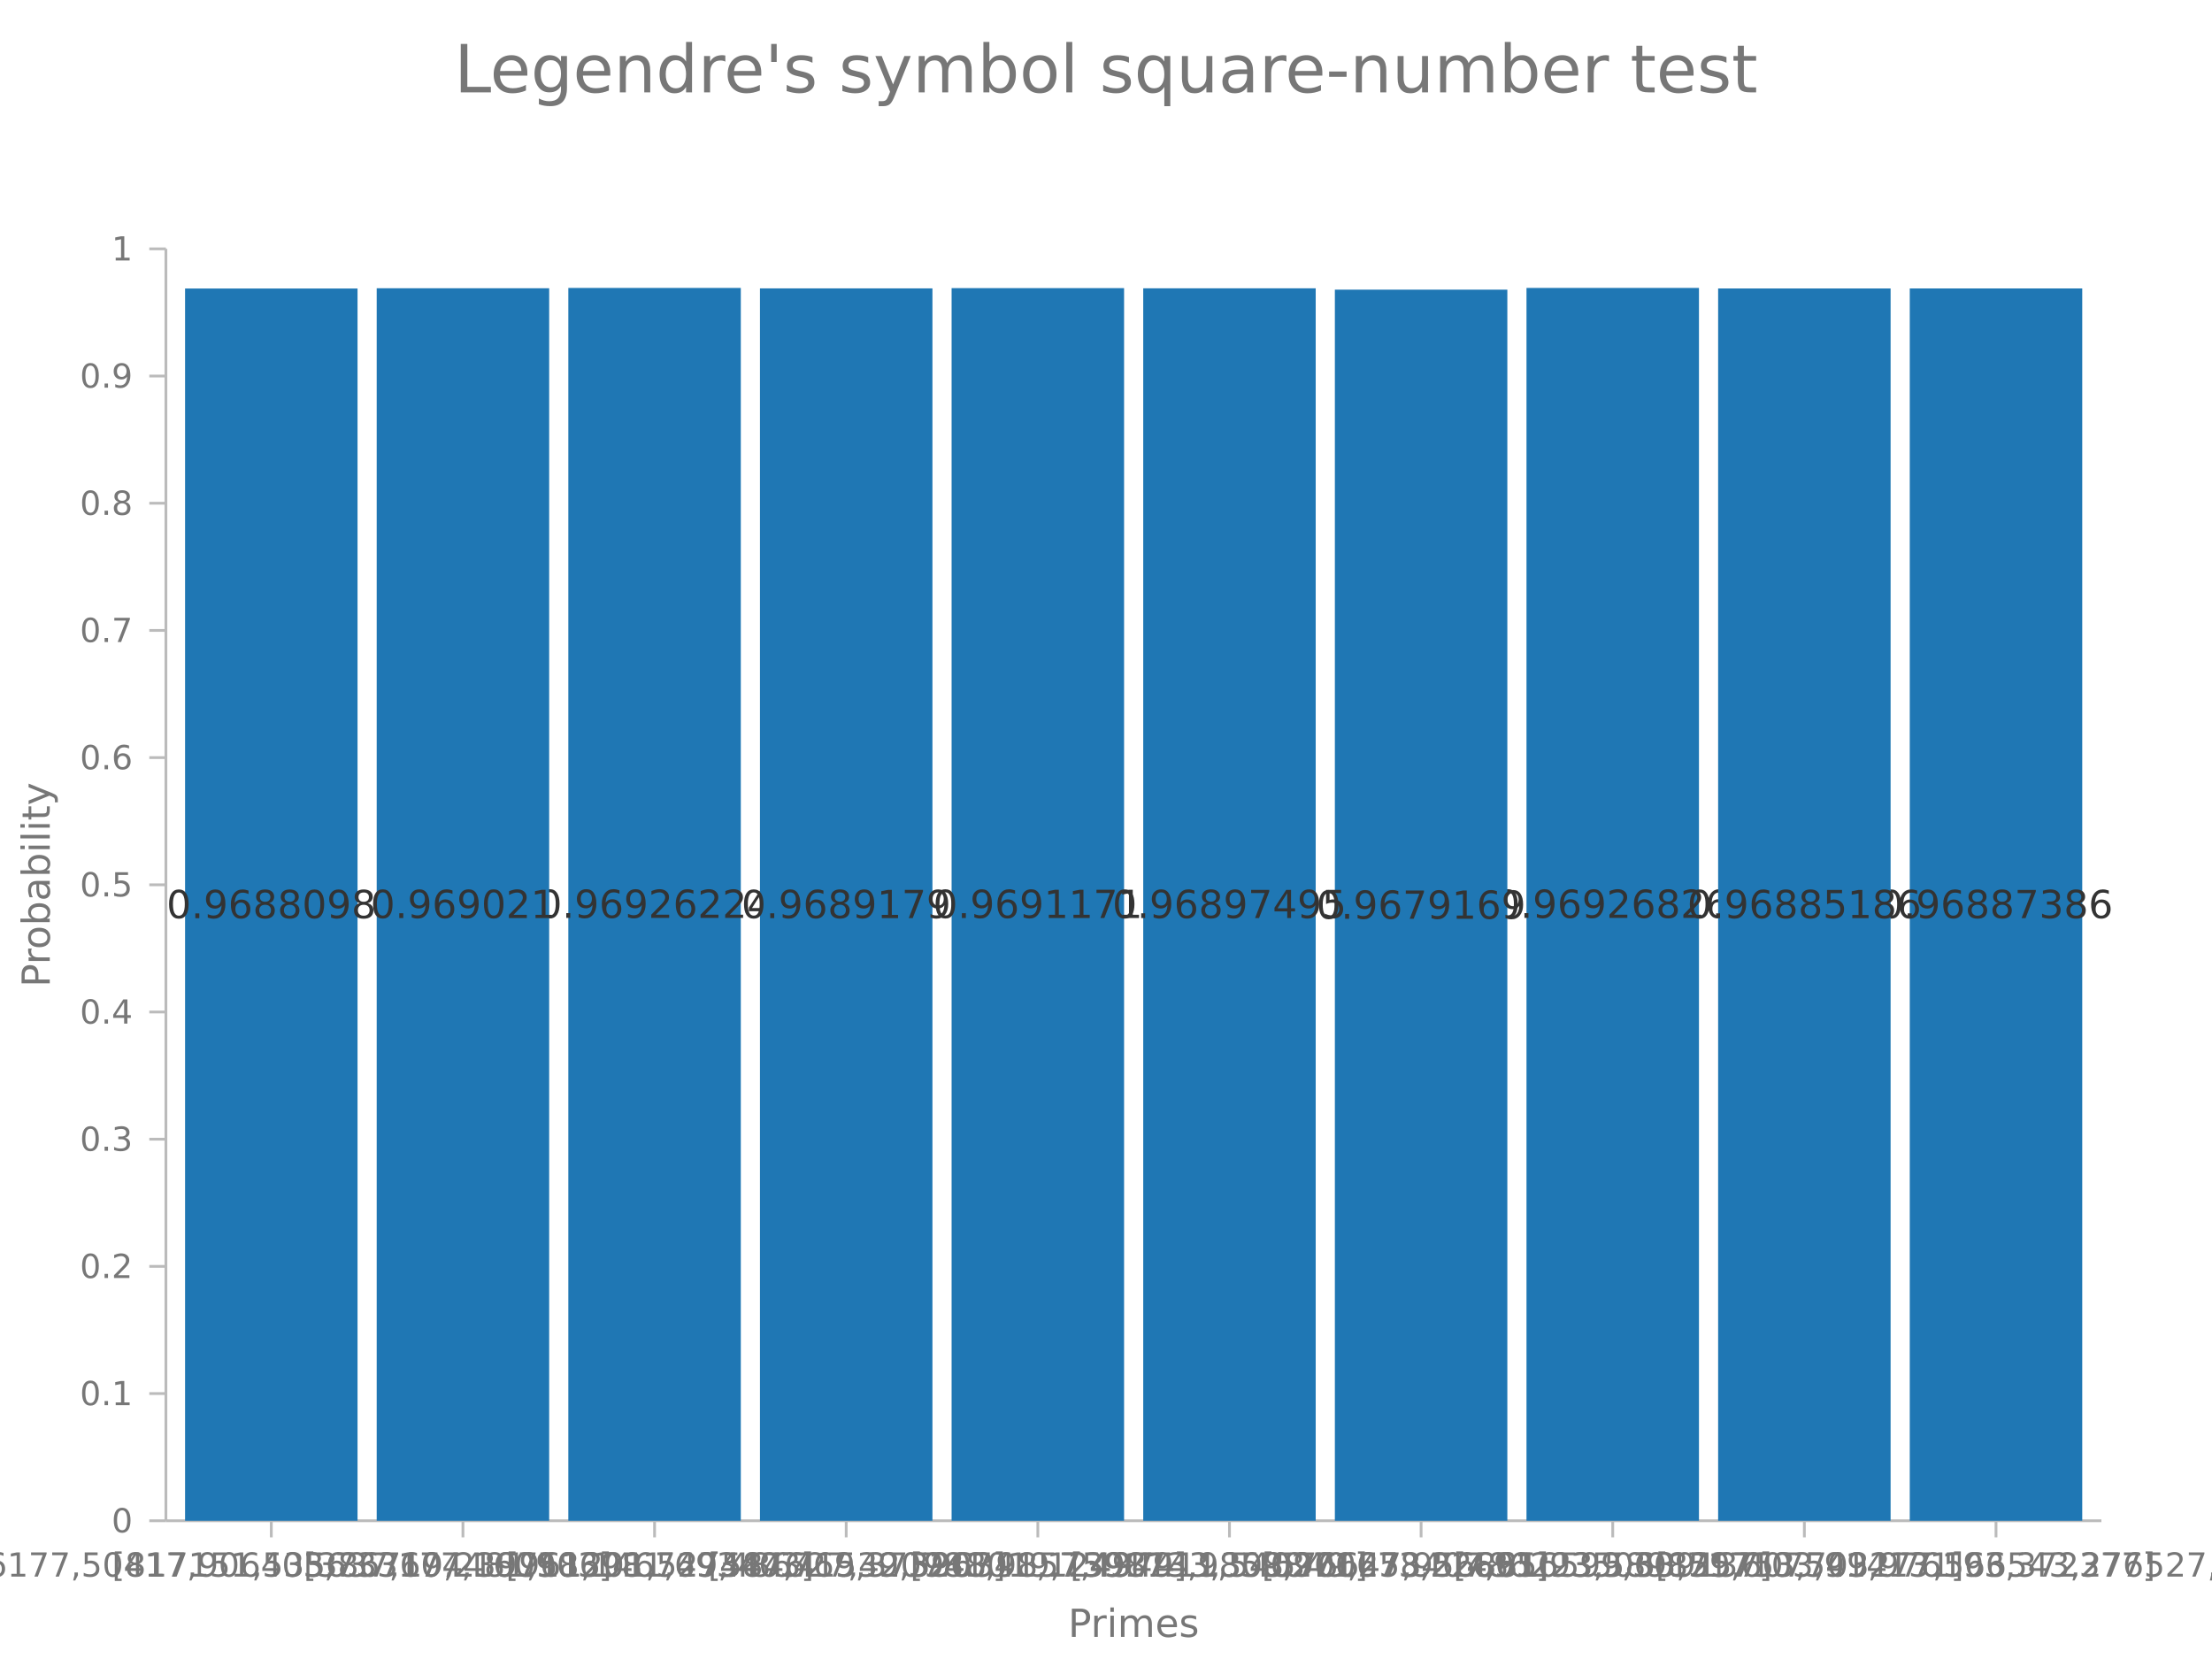
\includegraphics[width=\textwidth]{legendre-test-p.png}
            \caption{$|P|=5$로 일정할 때, 여러 $P$에 대하여 휴리스틱의 성공 확률을 나타낸 히스토그램.}
            \label{fig2}
        \end{figure}
        \ref{fig2}와 같은 수행 결과를 얻을 수 있었다.
    \section{결론}
        이와 같이 제곱수를 판정하는 정수론적인 휴리스틱을 제시하였다.
        하지만, 이를 통해서 완벽히 제곱수를 판정하는 것은 불가능하다.
        따라서, 추후 연구 방안으로 임의의 제곱수를 비트로 표현하였을 때 임의의 개수의 제곱수에 관하여 LCS(Longest-common-sequence)를 구하여 여기에서 찾은 LCS 를 통해서 매칭하는 휴리스틱을 제시하고, 위의 방법과 결합하여 더욱 판정률을 높인다.
    \newpage
    \begin{appendices}
        \section{휴리스틱 구현에 대한 소스코드}
            https://github.com/ANEP-Research/legendre-test 링크에 \texttt{Rust} 프로그래밍 언어를 통해서 휴리스틱과 테스트를 수행하는 코드를 볼 수 있다.
    \end{appendices}
    \bibliographystyle{acm}
    \bibliography{ref}
\end{document}